\documentclass[../../Thesis.tex]{subfiles}
\begin{document}
\header{Introduction and Background}
\subheader{Academic texts}
Academic texts are, among others, academic articles. These articles are focussed on specific domains, such as biology, economy and computer science, because of this, we call the articles "domain-specific" meaning that they give information about a topic in a domain (i.e. biology). Articles are published in journals, which are collections of articles which share a common topic, i.e. a specific field inside the biology domain. Our research focusses on the academic articles and journals not limited to a specific domain.
\subheader{Information retrieval}
Information Retrieval (IR) is the activity of gathering relevant information, starting from an initial piece of information. 
\\\\The most practical example of IR is a search engine. Given one or more search words (a query) the search engine will attempt to find relevant information. For example, an online search for "Information Retrieval" (initial piece of information) will return a list of results (relevant information). To be able to do return a list of results, the search engine must know which texts are related. \\\\Interpreting which texts are related can be achieved with, and without neural networks, a traditional technique which does not use a neural network is TF-IDF, shot for Term Frequency - Inverted Document Frequency. Techniques that use a neural network are (among others) Word2Vec, Paragraph Vectors and GloVe.

\subheader{Neural Networks}
A complete in-depth background into neural networks is beyond the scope of this thesis, therefore we will only describe the simplified working of neural networks and their basic application in IR.
Neural Networks are mathematical modesl\cite{funahashi1989approximate}, which use matrix transformations, to map input values to output values. This mapping uses a pre-defined amount of layers that modify the values through matrix transformations. Neural networks rely on training to create optimal values for these layers. Finding these optimal values is done iteratively, via a process known as "back-propagation". Back-propagation is done by starting at the output layer of the neural network and tracking the error in the output back through the layers. This error information is used to improve the values of the layers. The values of the layers are only changed at training time; high-quality (training) data is, therefore, essential for neural networks\cite{Truong2017Thesis, lai2016generate}. Neural networks can be applied to many different tasks, as long as there is sufficient data available to create a training and validation sets. During the training process, one seeks to achieve the optimal results, i.e. the result that is as close as possible to the given output for all input and output sets, without underperforming on other sets\footnote{Having only good results for the training/validation set is known as overfitting. This means that the layer-values are fine-tuned to only perform (extremely) well on one set while underperforming on others.}.\\Neural Networks are used, in the creation of word embeddings, to either predict words that may occur around a given word or predict a word given words that surround it. For example, given the sentence\\
\begin{center}
\textit{"The quick brown fox jumps over the lazy dog"}
\end{center}
a neural network can be trained to either predict the words around "jumps", which we refer to as context words (the, quick, brown, fox, over, the, lazy, dog), or to predict the word "jumps", given the context words (the, quick, brown, fox, over, the, lazy, dog). The training process results in a matrix, which is transformed to a collection of vectors, each vector is associated to a word, these vectors are referred to as word embeddings. This embedding indicates "word relatedness" which, as mentioned earlier enables association (thus retrieval) with related(relevant) texts. It is to be noted that the word embeddings are only able to represent word relatedness to the other words trained in the same run. Due to the random initialization of the initial values of the layers in  neural networks, the neural networks do not produce the same result every run. Therefore, word embeddings from different runs of the same neural network cannot be compared.


\subheader{Embedding}
An embedding is a distributed, numerical representation of text in a multi-dimensional vector space\footnote{The vector spaces of separately trained word embeddings differ, since each run the initial values of the neural network are randomly initialized. This means that the same word trained in two separate runs do not have to have the same embedding. However, they will have the same relationship to other words trained in their respective runs.} which can capture both semantic and syntactic information\cite{mikolov2013distributed}. In the case of word embeddings, the embeddings represent the words. These embeddings can be\footnote{This depends on the method used to create the word embeddings, for this research, we used word embeddings trained by an unsupervised learing algorithm.} created using machine learning models, which do not need human interaction~\cite{lai2016generate}, they are so-called \textit{unsupervised learning algorithms}. Once trained, the embeddings can also be used to construct embeddings for collections of texts. For example, a word embedding can be used to create sentence, paragraph, document or corpus embeddings. The usage of word embeddings has improved various Natural Language Processing areas such as named entity recognition, part-of-speech tagging, parsing, and semantic role labelling~\cite{luong2013better}. Embeddings can furthermore be used in search and recommendation. Potential application of the embeddings in the academic domain could be the improvement of search engines, text analysis to improve NLP tasks for academic texts, and journal recommendation for article publishing. The embeddings can furthermore be used to help researchers which are new to a field to explore the field by finding related articles or articles that are related to the field of expertise of the researcher and the new research field. Embeddings can also be visualized (see paragraph 1.6), this can give insight into the topics of popular journals, and can be used to indicate research subjects where there are few publications or journals.

\subheader{Text analysis techniques}
To enable a computer to process text, for embedding creation or other tasks, the text has to be processed by an algorithm. In this research, we used embeddings created by Word2Vec and feature vectors\footnote{Which do not require training (see subparagraph TF-IDF).} created using TF-IDF.
\begin{jumpin}
\subsubheader{Word2Vec}
Word2vec word embeddings are created using a neural network, Word2Vec learns word embeddings via maximizing the probability of the word given the context word(s) occurring within a fixed-sized window, therefore the learned embeddings contain useful knowledge about word co-occurrence\cite{nalisnick2016improving} which indicates relatedness\cite{lai2016generate}. There are multiple input/output possibilities for the neural network. The best known are Skip-gram and the Continuous Bag-of-Words model (CBOW). The Skip-gram model takes a target word as input and outputs the predicted context words, while CBOW takes the context words as input and outputs the predicted target word\cite{nalisnick2016improving, pennington2014glove}. This is illustrated in Figure~\ref{figure:word2vecModels}, where, $v(w)$ represents the target word, and $v(w...)$ represent the context words. \citet{mikolov2013distributed}\cite{mikolov2013efficient} presented several extensions to the word2vec model that improve the quality of the embeddings and the training speed, such as introducing Hierarchical Softmax, Negative Sampling and the subsampling of frequent words to the Skip-gram approach. Variations to the word2vec model have also been proposed, such as the doc2vec model described by \citet{lau2016empirical} which creates document embeddings\footnote{Document embeddings are embeddings which capture the relatedness between documents.} instead of word embeddings.

\begin{figure}[hbt]
\begin{center}
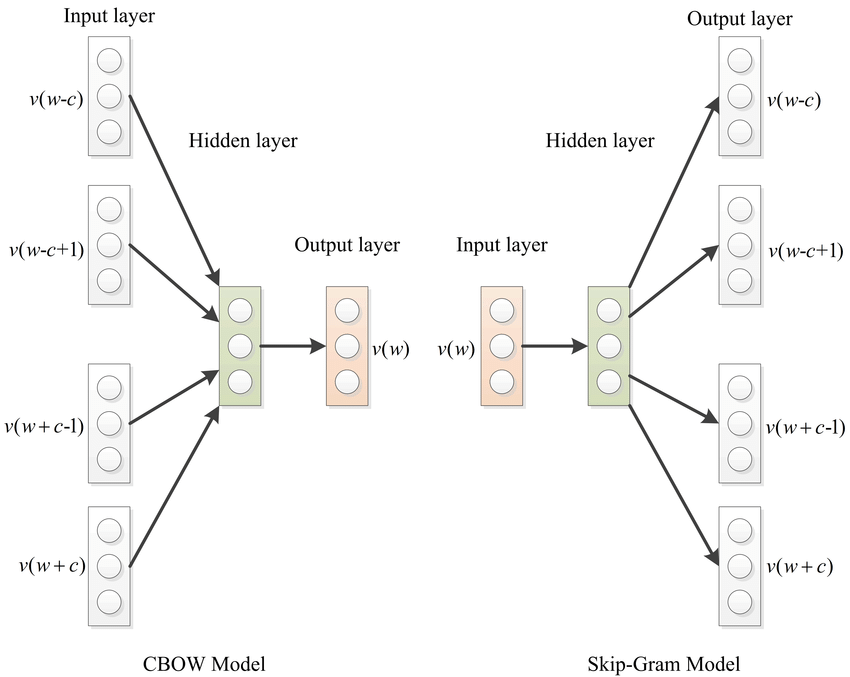
\includegraphics[width=4in]{Plots/Model-Architecture-of-CBOW-and-Skip-Gram.png}
\caption{Illustration of the CBOW and Skip-Gram models, as presented by \citet{chen2017convolutional}. Left part of the Figure illustrates the CBOW model, context words are represented at the left side (input) and the center word (output) is represented as $v(w)$ as output. The right side of the Figure illustrates the Skip-Gram Model, which takes the center word as input (left) and outputs the context words (right).}\label{figure:word2vecModels}
\end{center}
\end{figure}
\begin{figure}[hbt]
\begin{center}
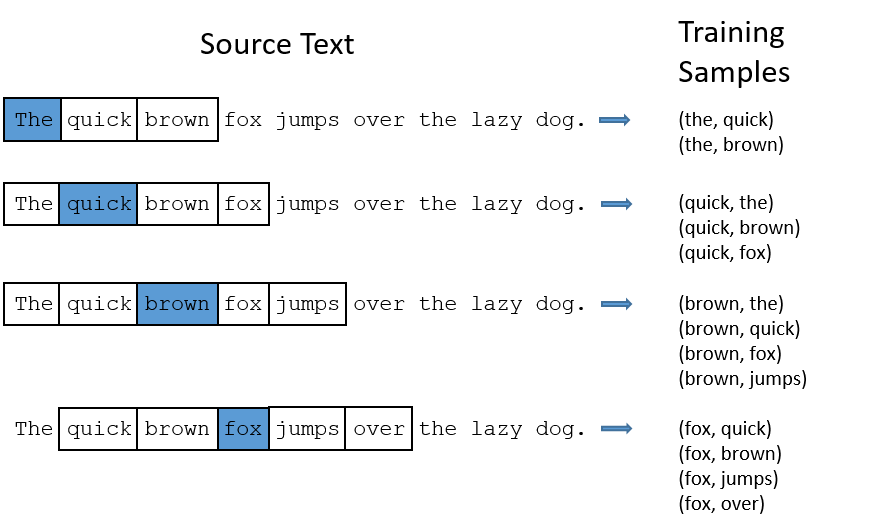
\includegraphics[width=4in]{Plots/training_window.png}
\caption{Illustration of the training windows. Illustration created by \citet{trainingWindow}.}
\end{center}
\end{figure}
\FloatBarrier
\subsubheader{Paragraph vectors}
Variations on the word2vec model have also been proposed,~\citet{le2014distributed} introduced the paragraph vector in their paper "Distributed representations of sentences and documents". The Paragraph Vector framework is based on the word vectors framework. The difference between the frameworks is the calculation of the probability, the Paragraph Vector framework uses a matrix, which consists of every paragraph. This matrix is used to replace a concatenation or average of word vectors. An advantage of the paragraph vector model is that it takes the word order into consideration, at least in a small context \cite{le2014distributed}. \citet{dai2015document} state that the Paragraph Vectors model performs significantly better than other models on grouping, triplet finding and related object/article finding tasks on Wikipedia and arXiv texts.

\subsubheader{GloVe}
\citet{pennington2014glove} introduced the Global Vectors (GloVe) model. This model captures the global corpus statistics. The model transforms the word co-occurrences of all words in the corpus to probabilities, it excludes all the zero probabilities and uses that as initial input for the neural network. This model outperforms other models on word analogy, word similarity and entity recognition according to the findings by~\citet{pennington2014glove}.\\

\subsubheader{TF-IDF}
Term Frequency * Inverted Document Frequency (TF-IDF) is a method that does not rely on a neural network and does not require training. The TF-IDF score is the product of the term frequency in a text and the inverted document frequency of the same term in a corpus of texts. Both of metrics, TF and IDF, can be calculated in a variety of ways. Table~\ref{table:TFIDFScore} shows an example of the TF-IDF calculation. The multiplication of the TF and IDF is referred to as the TF-IDF score. The text, provided to the algorithm, is analyzed on word occurrences on corpus and document level, resulting in one score per word. These scores (the scores of all words) can be converted to a feature vector, in which the indexes represent the words and the value is the TF-IDF score for the word. The size of this feature vector can optionally be controlled by hashing the words in the text. If hashing is not applied, the size of the feature vector is equal to the number of unique words in the corpus, also known as the (corpus) vocabulary.  The feature vectors produced by TF-IDF do not capture syntactic or semantic information about words, but capture information about word occurrences. Some applications of this technique limit the number of unique words in the text supplied to the TF-IDF algorithm, they do this by taking only a certain amount of top words, ordered on their occurrence. This reduces the amount of storage needed when hashing is not applied. It furthermore reduces the number of words which occur rarely. Due to the nature of TF-IDF, these rare words have a high score, canceling out other more frequent words, while rarely occurring in the corpus.
\vspace{0.3in}\begin{table}[hbt]
\begin{center}
\begin{tabular}{|p{1in}|R{1in}|R{1in}|R{1.3in}|R{1in}|}
\hline
Term & Frequency (TF) & Document Frequency (DF) & Inverted Document Frequency (IDF) & TF-IDF score\\
\hline
Exponential & 4 & 15 & 0.824 & 3.296\\
\hline
Occurrence & 1 & 20 & 0.699 & 0.699\\
\hline
Multitude & 1 & 40 & 0.398 & 0.398\\
\hline
Abstract & 100 & 100 & 0 & 0\\
\hline
\end{tabular}
\caption{Example of TF-IDF score calculation.}\label{table:TFIDFScore}
\end{center}
\end{table}
\FloatBarrier
\end{jumpin}
As \citet{lai2016generate} state in their paper "How to generate a good word embedding?", all embedding methods rely on the same hypothesis, \textit{words that occur in similar contexts have similar meanings}. They furthermore found that larger corpus lead to better quality embeddings, but that the domain in which the embeddings are trained has more influence on this than the corpus size. 
\subheader{Validation methods}
The results produced by the previously mentioned techniques have to be validated to determine their quality (in use). The quality of the results can be validated through various metrics. One of these is the F1 score\footnote{The F1 score combines the precision score and the recall score in a single metric.}. The embeddings can furthermore be validated through their performance on tasks such as word analogy, word similarity, categorization and embedding visualization. These tasks can be designed to produce a score that indicates the performance on a specific task. \citet{schnabel2015evaluation} found that a single validation metric cannot produce a representative result for other tasks. Embeddings that perform well on one task do not have to perform well on another task. As a result, the findings of the performance of an embedding method are limited to the task on which they are tested. Their results cannot be generalized to state that the embeddings are overall "performing well". Validation tasks use either labeled or unlabeled data. Labeled data is data that is in some way marked so that the correct answer can be derived from it, while this is not possible with unlabelled data. The validation tasks can be divided into two groups: extrinsic evaluation, i.e. tasks that use word embeddings as input for a downstream task, and Intrinsic evaluation, which directly tests the relationships of the word embeddings. \citet{schnabel2015evaluation} note that the extrinsic evaluation may not be consistent with intrinsic evaluations since the performance on downstream tasks is not consistent across tasks.
\clearpage
\begin{jumpin}
\subsubheader{Word Analogy}
Word analogy validation is based on a labelled validation set, containing word groups of four that can be logically divided into two parts. As Table~\ref{table:wordAnalogies} shows, each last word can be derived from the three words before. The score is the fraction of correctly given fourth words, given the first three words. This validation metric is used in multiple studies\cite{mikolov2013distributed, mikolov2013efficient, dai2015document, pennington2014glove}.\\
\begin{table}[hbt]
\begin{center}
\begin{tabular}{|l|l||l|l|}
\hline
\textbf{Word 1} & \textbf{Word 2} & \textbf{Word 3} & \textbf{Word 4}\\
\hline
\hline
Man & Woman & King & Queen \\
\hline
Athens & Greece & Oslo & Norway\\
\hline
Great & Greater & Tough & Tougher\\
\hline
\end{tabular}
\end{center}
\caption{Word analogies examples}\label{table:wordAnalogies}
\end{table}\\
Both this validation technique and the Word Similarity technique use vector distance calculations to validate the embeddings, the word group can therefore also be written as:
\begin{displayquote}
    X\textsubscript{King} - X\textsubscript{Man} $\approx$  X\textsubscript{Queen} - X\textsubscript{Woman}
\end{displayquote}
This means that the resulting vector of embedding of "King" minus the embedding of "Men" is approximately the embedding of "Queen" minus the embedding of "Woman". The resulting vector of the subtraction may, for example, be close to the vector of the embedding for "Monarch".
\subsubheader{Word Similarity}
A method to test the quality of word embeddings is the word similarity test. For this test, the distance between the word embeddings (vectors) is measured and compared to similarity scores defined by humans. Multiple non-domain specific validation sets are publicly available including the Rare-word dataset introduced in the paper "Better Word Representations with Recursive Neural Networks for Morphology" by \citet{luong2013better}, 
the MEN test collection by \citet{EBruniMENCollection} and the WordSimilarity-353 test collection by \citet{EGabrilovichWScollection}.
These sets, among others, have been used in multiple studies of word embeddings\cite{pennington2014glove, mikolov2013efficient}. This validation method is limited by the availability of word similarity sets that share the same domain as the trained embeddings.
\subsubheader{Classification}
A classification validation method is a simple task which assigns a label to a text. \citet{lau2016empirical} used text pairs from StackExchange and tried to determine if a pair was a duplicate. In their setup the categories were duplicate and non-duplicate. \citet{le2014distributed} used for their research a dataset of IMDB with 100,000 movie reviews. They validated their proposed paragraph vector model by determining whether a review was positive or negative. We will use the classification task for our research too, we will use journals (collection of articles) as classes, and the articles as items that need to be classified. We create a list, sorted on the similarity between article and journal, of journals for each article to get a measurable ranking result. From the resulting list we can extract, among other things, the position (rank) of the journal from which the article was taken.
\subsubheader{Position Visualization}
\citet{dai2015document} and \citet{hinton2003stochastic} mapped their word embeddings from a high dimensional vector to a two-dimensional vector to be able to display them in a scatter plot and apply colors to various categories. The advantage of this visualization is that a human can directly see the embedding distribution, and see if it is distributed in a way that seems logical. It gives furthermore insight in the overall spectrum of the embedding. However, this representation does not give an empirical score, since it is not an evaluation of the data, but an alternative representation. 
\end{jumpin}
\clearpage
\subheader{General and Domain specific}
Since the word embeddings are created from a given text, these embeddings are bound to the text. All meaning embedded in the word embedding is derived from the original text, therefore embeddings can be "domain-specific" meaning that some words are only known in a certain context. This becomes most clear when faced with words that can have different meanings in different contexts. For this research, we categorize the embeddings into two categories, generic embeddings and domain-specific embeddings. The generic embeddings are trained on a collection of texts that use common English and contains a wide variety of topics. The domain-specific embeddings are trained on a collection of texts that uses jargon English (i.e., domain-specific terminology) or is limited to a small number of topics. Given these terms, we regard the embeddings trained on the Wikipedia corpus\cite{lai2016generate, pennington2014glove, dai2015document, lau2016empirical, schnabel2015evaluation} as general, since Wikipedia uses common English and spans a wide range of topics. On the other hand, we regard the embeddings created by \citet{Truong2017Thesis} as Domain specific; these embeddings were created on academic articles, which use domain-specific terms and notations and only consists of academic texts, which contains less general/generic words compared to the Wikipedia corpus. Figure~\ref{figure:domainPlot} illustrates our corpus, marked in green, in comparison to the Wikipedia corpus, marked in blue. Our corpus is a collection of domain-specific texts, written in academic language. A set that would be more specific would only focus on the individual domains or sub-domains.
\begin{figure}[hbt]
\begin{center}
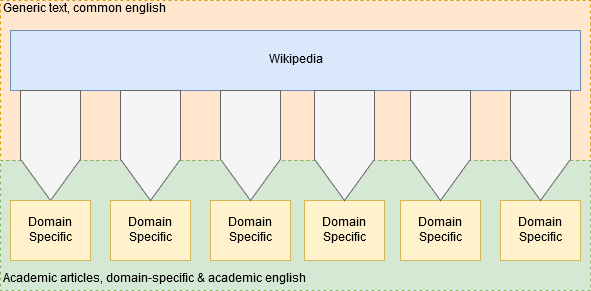
\includegraphics[width=4.5in]{Plots/domain_specification_graph}
\caption{Illustration of generic texts and domain-specific texts. Our research focusses on the green-marked area.}\label{figure:domainPlot}
\end{center}
\end{figure}
\subheader{Domain-specific \& in-domain}
In this paragraph, we will explain the meaning of the term "in-domain". The term domain-specific refers to a specific domain, i.e. biology or chemistry. In-domain refers to a relation between texts, meaning that an article on biology is an in-domain text of another article on biology, but not on an article on chemistry. This means that two domain-specific texts do not necessarily share their domain, while a text A which is an in-domain text for text B means that text A and B share the same domain.
\end{document}